\section{Background}
\label{sec:background}
%\shuqing{Maybe we could introduce HID devices somewhere.}
%\noindent\outline{USB Standard}\\

We first introduce the development of \ac{USB} specification and emphasize the key
points adopted in this work. We also organized a brief timeline for introducing
key points of each protocol in Table~\ref{table:usb_timeline}.

%\noindent\outline{USB1.x}\\
Proposed in 1996, \ac{USB} 1.0~\cite{usb10} was developed to provide a unified
interface and thus reducing the cost of reconfiguring the software. It is
worth mentioning that as a polled-bus interface, all data transfers are
initiated by the host.

%\noindent\outline{HID Protocol}\\
Right after one year of the appearance of \ac{USB} 1.0, a standard named \acf{HID}~\cite{hid} was designed based on \ac{USB}. \ac{HID} is
designed to unify the implementation for devices like mice,
keyboards, etc. Before its appearance, the standard is divided among
manufacturers, for example, the mouse of Company A may use X-Y coordinates to
represent its location while the mouse of Company B uses relative displacement.
This means every device needs its own driver to work. After \ac{HID}, users only need to
write one driver for an entire class of \acp{HID}. Furthermore, the \ac{HID} standard also
requires all devices to be \ac{PnP}, which is indeed
convenient but insecure too.

In 1998, the first widely supported \ac{USB} protocol was designed. \ac{USB} 1.1~\cite{usb11}
provided two data transfer rates which are low speed (1.5 Mbit/s) and full
speed (12 MBit/s). At this point, due to the transfer limitation, it only supports
limited types of devices like keyboards, mice, etc.

%\noindent\outline{USB2.0}\\
In 2000, the \ac{USB} 2.0~\cite{usb20} specification was released. With high speed \mbox{(480
Mbit/s)} mode introduced, printers, cameras, CD-ROM drives, and network cards were
supported in this revision. Such a high data transfer rate also gave rise to the
popularity of ``flash drive'', a portable device that allows physically
transferring data around~\cite{sok}. Although various peripherals were supported
in \ac{USB} 2.0, there was no reliable way to identify the type of device. This
security flaw allowed attacks like BadUSB~\cite{badusb,rubber}.

%\noindent\outline{USB3.x}\\
\ac{USB} 3.0~\cite{usb30} was introduced in 2008, with a super speed \mbox{(5 Gbit/s)} data
transfer rate. Like its predecessor, more classes of peripherals were supported
in this revision. In 2013, the \ac{USB} Type-C connector standard was introduced as a
part of \ac{USB} 3.1~\cite{usb31}, providing a unified connector type for
PowerDelivery, Thunderbolt, DisplayPort, and HDMI.  Yet no improvement of
security was introduced in 3.x revisions, meaning any device claiming
itself as a monitor can capture the video stream from the host. Exposing
such a multi-purpose connector unprotected is insecure and allows attacks similar to \tool. In 2017, \ac{USB} 3.2~\cite{usb32} was released, doubling the data
transfer rate (20 Gbit/s).

%\noindent\outline{Connector Standard}
\begin{figure}[t]
    \centering
	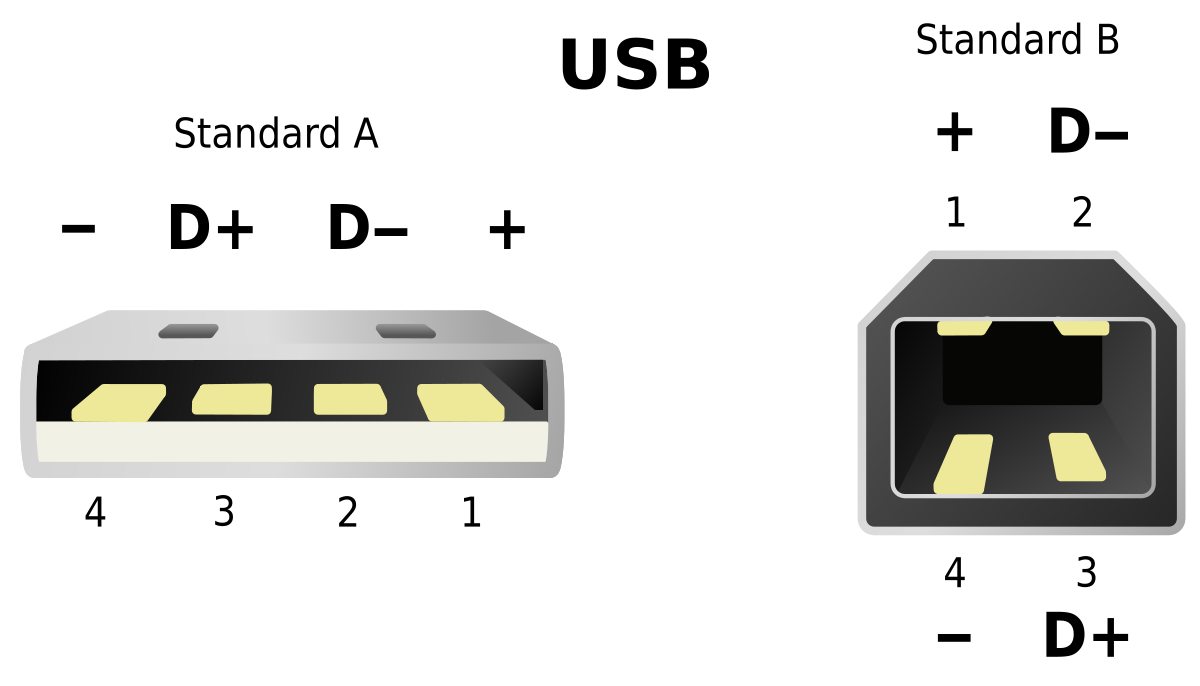
\includegraphics[width=0.7\linewidth]{./Figs/usb_conn.png}
	\caption{\ac{USB} 1.x \& 2.x Connector.}
	\label{fig:usb_conn}
\end{figure}

As illustrated in Figure~\ref{fig:usb_conn}, the original \ac{USB} 1.x \& 2.x
connector only has two pins for data transferring \mbox{(D+ \& D-)}, which has
significantly limited data transfer rate \mbox{(5 Gbits/s Max)} and cannot support
peripherals like DisplayPort \mbox{(10.8 Gbit/s Min)}. Apart from that, support for
other peripherals also requires dedicated transferring lanes as their standards
are not compatible with \ac{USB} in most cases.  

\begin{figure}[t] 
	\centering
	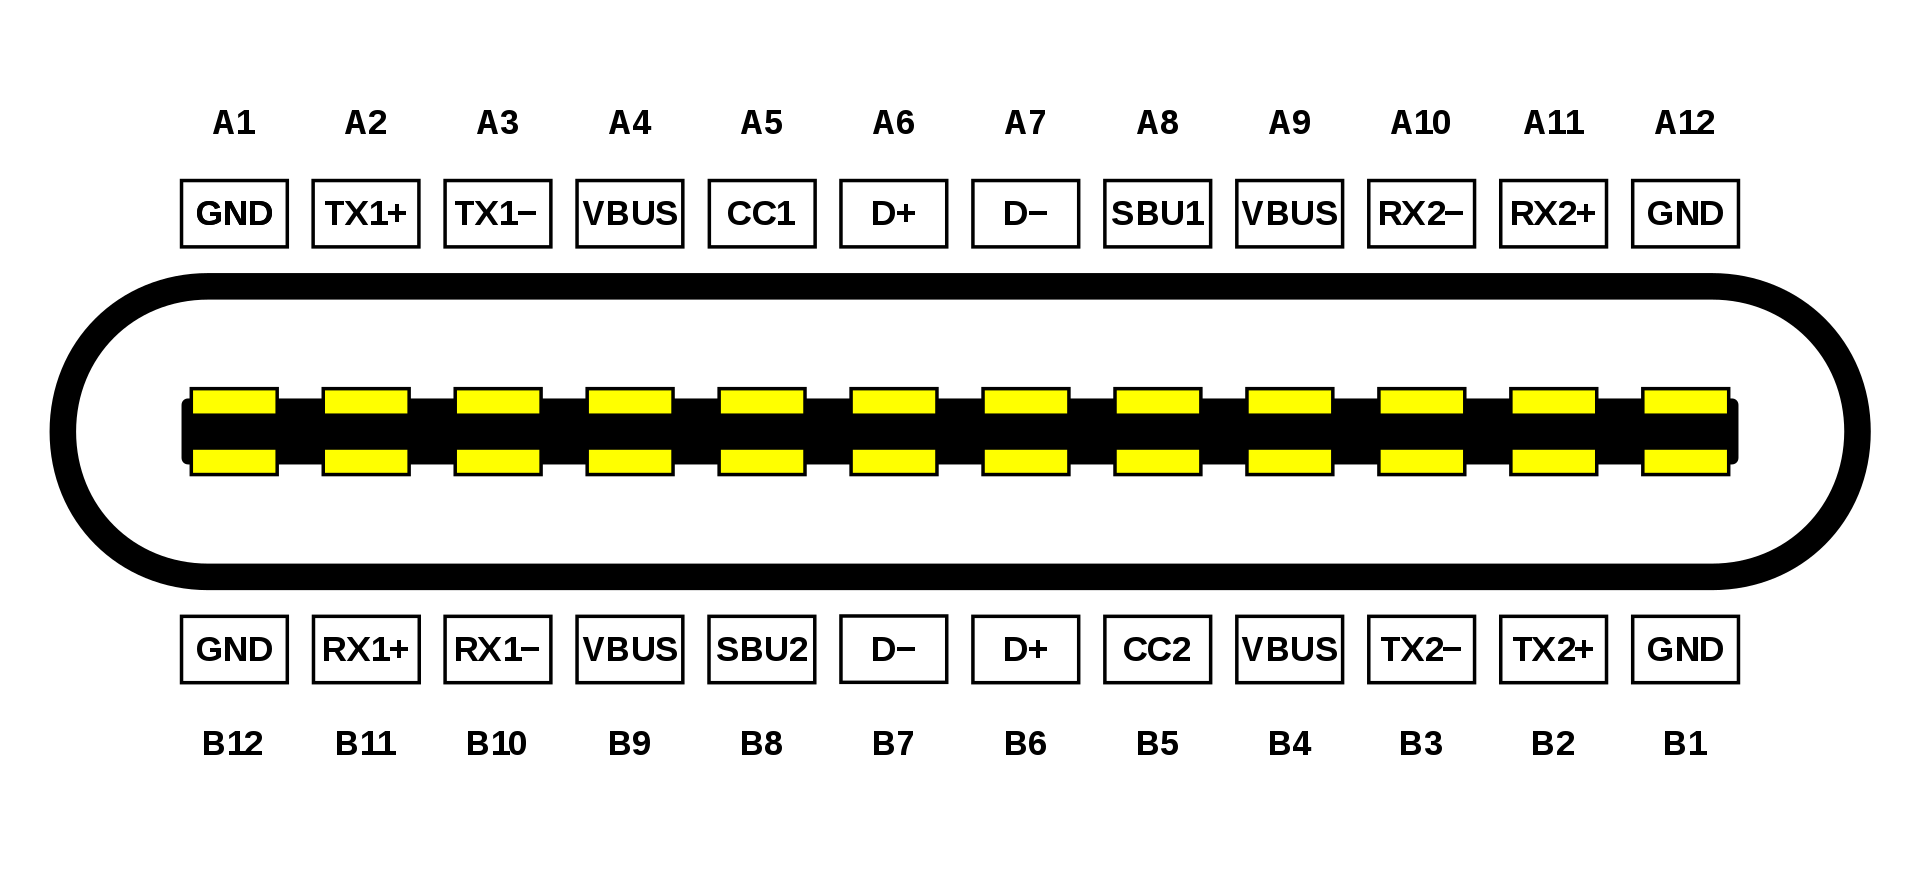
\includegraphics[width=\linewidth]{./Figs/usb_c_conn.png} 
	\caption{\ac{USB} Type-C Connector.} 
	\label{fig:usb_c_conn} 
\end{figure}

Thus, to provide support towards a wider range of peripherals, a 24-pins
standard called \ac{USB} Type-C~\cite{typec} was introduced in 2013 by \ac{USB}-IF~\cite{usbif}. As it is designed to be double-sided, the number of actually usable
pins is halved. Nevertheless, this standard has largely enhanced the capability
of the \ac{USB} 3.x protocol. As presented in Figure~\ref{fig:usb_c_conn}, Type-C added
two high-speed data lanes \mbox{(TRX1 \& TRX2)} and kept the original data lane \mbox{(D+ \&
D-)}. The added lanes are used exclusively to support peripherals like
DisplayPort while the kept data lane transfers \ac{USB} packets.

%\noindent\outline{Security Problem}\\
During the development of the \ac{USB} specification, security was insufficiently considered~\cite{sok}. 
The \ac{USB}-IF believes it is the duty of \acp{OEM}
to decide whether security features should be implemented~\cite{usbsec}. But the divergent implementations give a chance for attacks like
BadUSB~\cite{rubber} and our \tool.

%\fengwei{FIXME: add a reference for each attack in the Table.}
%\fengwei{FIXME: The table is too wide, exceeds the max size.}
\begin{table*}
\begin{tabular}{|c|l|c|c|c|}
	\hline
	\textbf{Year} & \textbf{Protocol Version} & \textbf{Supported Peripherals} & \textbf{Transfer Speed} & \textbf{Attacks} \\
	\hline
	1996 & \ac{USB} 1.x~\cite{usb10,usb11} & Keyboard, Mouse... & 1.5 Mbit/s or 12 Mbit/s & \ac{HID} Emulation (BadUSB)~\cite{badusb} \\
	\hline
	2000 & \ac{USB} 2.0~\cite{usb20} & Flash Drive, High-Definition Link, CD Driver... & 480 Mbit/s & Autorun Attack~\cite{duqu}, Juice Filming~\cite{JFC,JFCImpact} \\
	\hline
	2008 & \ac{USB} 3.0~\cite{usb30} & / & 5 Gbit/s & / \\
	\hline
	2013 & \ac{USB} 3.1~\cite{usb31} & HDMI, DisplayPort, ThunderBolt... & 10 Gbit/s & \tool \\
	\hline
	2017 & \ac{USB} 3.2~\cite{usb32} & / & 20 Gbit/s & / \\
	\hline
\end{tabular}
	\linebreak
\caption{\ac{USB} Protocol Timeline.}
\label{table:usb_timeline}
\end{table*}
